\documentclass[10pt]{article}
\usepackage[letterpaper,margin=0.72in,headheight=15pt]{geometry}
\usepackage[T1]{fontenc}
\usepackage{sourcesans}
\usepackage{microtype}
\usepackage{booktabs}
\usepackage{array}
\usepackage{tabularx}
\usepackage{graphicx}
\usepackage{xcolor}
\usepackage{fancyhdr}
\usepackage{titlesec}
\usepackage{enumitem}
\usepackage{tikz}
\usetikzlibrary{arrows.meta,positioning,shapes.geometric}
\usepackage[hidelinks]{hyperref}
\newcommand{\NumCaptures}{144}
\newcommand{\NumQASamples}{16}
\newcommand{\NumSummarySamples}{8}
\newcommand{\QATwoUploadReductionTLS}{54}
\newcommand{\QAFourUploadReductionTLS}{76}
\newcommand{\QATwoTotalReductionTLS}{51}
\newcommand{\QAFourTotalReductionTLS}{71}
\newcommand{\SummaryTwoUploadReductionTLS}{38}
\newcommand{\SummaryFourUploadReductionTLS}{55}
\newcommand{\SummaryTwoTotalReductionTLS}{6}
\newcommand{\SummaryFourTotalReductionTLS}{20}
\newcommand{\TokenUploadCorrelationTLS}{0.88}
\newcommand{\TokenUploadCorrelationQUIC}{0.88}

\usepackage{pgfplots}
\usepgfplotslibrary{groupplots,statistics,fillbetween}
\pgfplotsset{compat=1.18}

\definecolor{AIBlue}{HTML}{0072B2}
\definecolor{AIOrange}{HTML}{D55E00}
\definecolor{AIGreen}{HTML}{009E73}
\definecolor{AIPurple}{HTML}{7B61A8}
\definecolor{AIGray}{HTML}{6B7280}
\definecolor{AIGrid}{HTML}{E5E7EB}

\pgfplotsset{
  conference/.style={
    width=0.93\linewidth,
    height=0.56\textheight,
    axis line style={draw=AIGray},
    tick style={draw=AIGray},
    grid=major,
    grid style={draw=AIGrid,line width=0.35pt},
    tick label style={font=\scriptsize},
    label style={font=\small},
    title style={font=\small\bfseries},
    legend style={
      draw=none,
      fill=none,
      font=\scriptsize,
      /tikz/every even column/.append style={column sep=0.8em}
    },
    every axis plot/.append style={line width=1.2pt},
    unbounded coords=discard,
  },
  conference bar/.style={
    conference,
    ybar,
    bar width=8pt,
    enlarge x limits=0.22,
    nodes near coords,
    nodes near coords style={font=\tiny,/pgf/number format/fixed,/pgf/number format/precision=0},
    legend columns=-1,
  },
}

\newcommand{\PlotTokenMedians}{
\begin{tikzpicture}
\begin{axis}[
  conference bar,
  xtick={0,1,2},
  xticklabels={Original,2x,4x},
  ylabel={Median input tokens (thousands)},
  ymin=0,
  ymax=52,
  legend style={at={(0.5,1.02)},anchor=south,legend columns=-1},
]
\addplot+[fill=AIBlue,draw=AIBlue] table[x=x,y=qa_k,col sep=comma]
  {figures/data/plot_token_medians.csv};
\addplot+[fill=AIOrange,draw=AIOrange] table[x=x,y=summary_k,col sep=comma]
  {figures/data/plot_token_medians.csv};
\legend{QA,Event summary}
\end{axis}
\end{tikzpicture}
}

\newcommand{\ReductionPlot}[2]{
\begin{tikzpicture}
\begin{groupplot}[
  group style={group size=2 by 1,horizontal sep=1.25cm},
  conference bar,
  width=0.46\linewidth,
  height=0.54\textheight,
  xtick={0,1},
  xticklabels={2x,4x},
  ylabel={Median reduction (\%)},
  ymin=0,
  ymax=85,
  legend style={at={(0.5,1.16)},anchor=south,legend columns=-1},
  error bars/y dir=both,
  error bars/y explicit,
]
\nextgroupplot[title={QA}]
\addplot+[fill=AIBlue,draw=AIBlue] table[
  x=x,y=qa_tls13,y error plus=qa_tls13_err_plus,y error minus=qa_tls13_err_minus,col sep=comma]
  {#1};
\addplot+[fill=AIOrange,draw=AIOrange] table[
  x=x,y=qa_http3,y error plus=qa_http3_err_plus,y error minus=qa_http3_err_minus,col sep=comma]
  {#1};
\legend{TLS 1.3,HTTP/3}
\nextgroupplot[title={Event summary},ylabel={}]
\addplot+[fill=AIBlue,draw=AIBlue] table[
  x=x,y=summary_tls13,y error plus=summary_tls13_err_plus,y error minus=summary_tls13_err_minus,col sep=comma]
  {#1};
\addplot+[fill=AIOrange,draw=AIOrange] table[
  x=x,y=summary_http3,y error plus=summary_http3_err_plus,y error minus=summary_http3_err_minus,col sep=comma]
  {#1};
\end{groupplot}
\end{tikzpicture}
}
\newcommand{\PlotUploadReduction}{
  \ReductionPlot{figures/data/plot_upload_reduction.csv}{Client-to-server bytes}
}
\newcommand{\PlotTotalReduction}{
  \ReductionPlot{figures/data/plot_total_reduction.csv}{Bidirectional frame bytes}
}
\newcommand{\PlotLatencyReduction}{
  \ReductionPlot{figures/data/plot_latency_reduction.csv}{End-to-end generation latency}
}

\newcommand{\DirectionPlot}[2]{
\begin{tikzpicture}
\begin{axis}[
  conference,
  ybar stacked,
  bar width=15pt,
  width=0.96\linewidth,
  height=0.56\textheight,
  xtick={0,1,2,4,5,6},
  xticklabels={TLS Orig.,TLS 2x,TLS 4x,H3 Orig.,H3 2x,H3 4x},
  xticklabel style={rotate=22,anchor=east,font=\scriptsize},
  ylabel={Median captured bytes (KiB)},
  ymin=0,
  legend style={at={(0.5,1.02)},anchor=south,legend columns=-1},
]
\addplot+[fill=AIBlue,draw=AIBlue] table[x=x,y=upload_kib,col sep=comma]{#1};
\addplot+[fill=AIOrange,draw=AIOrange] table[x=x,y=download_kib,col sep=comma]{#1};
\legend{Client $\rightarrow$ server,Server $\rightarrow$ client}
\end{axis}
\end{tikzpicture}
}
\newcommand{\PlotDirectionQA}{
  \DirectionPlot{figures/data/plot_direction_qa.csv}{QA is upload dominated}
}
\newcommand{\PlotDirectionSummary}{
  \DirectionPlot{figures/data/plot_direction_summary.csv}{Summary traffic is output dominated}
}

\newcommand{\PlotProtocolBytes}{
\begin{tikzpicture}
\begin{axis}[
  conference bar,
  xtick={0,1,2},
  xticklabels={Original,2x,4x},
  ylabel={HTTP/3 / TLS total-byte ratio},
  ymin=0.85,
  ymax=1.12,
  nodes near coords style={font=\tiny,/pgf/number format/fixed,/pgf/number format/precision=2},
  legend style={at={(0.5,1.02)},anchor=south,legend columns=-1},
]
\addplot+[fill=AIBlue,draw=AIBlue] table[x=x,y=qa_bytes,col sep=comma]
  {figures/data/plot_protocol_ratio.csv};
\addplot+[fill=AIOrange,draw=AIOrange] table[x=x,y=summary_bytes,col sep=comma]
  {figures/data/plot_protocol_ratio.csv};
\addplot[AIGray,dashed,sharp plot,forget plot] coordinates {(-0.5,1) (2.5,1)};
\legend{QA,Event summary}
\end{axis}
\end{tikzpicture}
}

\newcommand{\PlotProtocolPackets}{
\begin{tikzpicture}
\begin{axis}[
  conference bar,
  xtick={0,1,2},
  xticklabels={Original,2x,4x},
  ylabel={HTTP/3 / TLS packet-count ratio},
  ymin=0,
  ymax=3.3,
  nodes near coords style={font=\tiny,/pgf/number format/fixed,/pgf/number format/precision=2},
  legend style={at={(0.5,1.02)},anchor=south,legend columns=-1},
]
\addplot+[fill=AIBlue,draw=AIBlue] table[x=x,y=qa_packets,col sep=comma]
  {figures/data/plot_protocol_ratio.csv};
\addplot+[fill=AIOrange,draw=AIOrange] table[x=x,y=summary_packets,col sep=comma]
  {figures/data/plot_protocol_ratio.csv};
\addplot[AIGray,dashed,sharp plot,forget plot] coordinates {(-0.5,1) (2.5,1)};
\legend{QA,Event summary}
\end{axis}
\end{tikzpicture}
}

\newcommand{\PlotLatencyMedians}{
\begin{tikzpicture}
\begin{groupplot}[
  group style={group size=2 by 1,horizontal sep=1.2cm},
  conference,
  width=0.46\linewidth,
  height=0.54\textheight,
  xtick={0,1,2},
  xticklabels={Original,2x,4x},
  ylabel={Median latency (s)},
  ymin=0,
  legend style={at={(0.5,1.16)},anchor=south,legend columns=-1},
]
\nextgroupplot[title={QA},ymax=10]
\addplot+[mark=*,color=AIBlue] table[x=x,y=qa_tls13,col sep=comma]{figures/data/plot_latency_medians.csv};
\addplot+[mark=square*,color=AIOrange] table[x=x,y=qa_http3,col sep=comma]{figures/data/plot_latency_medians.csv};
\legend{TLS 1.3,HTTP/3}
\nextgroupplot[title={Event summary},ylabel={},ymax=28]
\addplot+[mark=*,color=AIBlue] table[x=x,y=summary_tls13,col sep=comma]{figures/data/plot_latency_medians.csv};
\addplot+[mark=square*,color=AIOrange] table[x=x,y=summary_http3,col sep=comma]{figures/data/plot_latency_medians.csv};
\end{groupplot}
\end{tikzpicture}
}

\newcommand{\PlotAbsoluteTotal}{
\begin{tikzpicture}
\begin{groupplot}[
  group style={group size=2 by 1,horizontal sep=1.2cm},
  conference bar,
  width=0.46\linewidth,
  height=0.54\textheight,
  xtick={0,1,2},
  xticklabels={Original,2x,4x},
  ylabel={Median total traffic (KiB)},
  ymin=0,
  legend style={at={(0.5,1.16)},anchor=south,legend columns=-1},
]
\nextgroupplot[title={QA},ymax=180]
\addplot+[fill=AIBlue,draw=AIBlue] table[x=x,y=qa_tls13,col sep=comma]{figures/data/plot_total_kib.csv};
\addplot+[fill=AIOrange,draw=AIOrange] table[x=x,y=qa_http3,col sep=comma]{figures/data/plot_total_kib.csv};
\legend{TLS 1.3,HTTP/3}
\nextgroupplot[title={Event summary},ylabel={},ymax=430]
\addplot+[fill=AIBlue,draw=AIBlue] table[x=x,y=summary_tls13,col sep=comma]{figures/data/plot_total_kib.csv};
\addplot+[fill=AIOrange,draw=AIOrange] table[x=x,y=summary_http3,col sep=comma]{figures/data/plot_total_kib.csv};
\end{groupplot}
\end{tikzpicture}
}

\newcommand{\PlotTokenUploadScatter}{
\begin{tikzpicture}
\begin{groupplot}[
  group style={group size=2 by 1,horizontal sep=1.2cm},
  conference,
  width=0.46\linewidth,
  height=0.54\textheight,
  xlabel={Input tokens},
  ylabel={Client-to-server traffic (KiB)},
  xmin=0,
  ymin=0,
  legend style={at={(0.5,1.16)},anchor=south,legend columns=-1},
]
\nextgroupplot[title={TLS 1.3}]
\addplot+[only marks,mark=*,mark size=1.7pt,color=AIBlue,opacity=0.72]
  table[x=input_tokens,y=upload_kib,col sep=comma]{figures/data/scatter_qa_tls13.csv};
\addplot+[only marks,mark=triangle*,mark size=2pt,color=AIOrange,opacity=0.72]
  table[x=input_tokens,y=upload_kib,col sep=comma]{figures/data/scatter_summary_tls13.csv};
\legend{QA,Event summary}
\nextgroupplot[title={HTTP/3},ylabel={}]
\addplot+[only marks,mark=*,mark size=1.7pt,color=AIBlue,opacity=0.72]
  table[x=input_tokens,y=upload_kib,col sep=comma]{figures/data/scatter_qa_http3.csv};
\addplot+[only marks,mark=triangle*,mark size=2pt,color=AIOrange,opacity=0.72]
  table[x=input_tokens,y=upload_kib,col sep=comma]{figures/data/scatter_summary_http3.csv};
\end{groupplot}
\end{tikzpicture}
}

\newcommand{\PlotTotalECDF}{
\begin{tikzpicture}
\begin{groupplot}[
  group style={group size=2 by 1,horizontal sep=1.2cm},
  conference,
  width=0.46\linewidth,
  height=0.54\textheight,
  xlabel={Compressed / original total bytes},
  ylabel={Fraction of paired samples},
  xmin=0.2,
  xmax=1.2,
  ymin=0,
  ymax=1.02,
  legend style={at={(0.5,1.16)},anchor=south,legend columns=2},
]
\nextgroupplot[title={QA}]
\addplot+[color=AIBlue,solid] table[x=ratio,y=ecdf,col sep=comma]
  {figures/data/ecdf_qa_tls13_longllmlingua_2x.csv};
\addlegendentry{TLS 2$\times$}
\addplot+[color=AIOrange,solid] table[x=ratio,y=ecdf,col sep=comma]
  {figures/data/ecdf_qa_tls13_longllmlingua_4x.csv};
\addlegendentry{TLS 4$\times$}
\addplot+[color=AIBlue,dashed] table[x=ratio,y=ecdf,col sep=comma]
  {figures/data/ecdf_qa_http3_longllmlingua_2x.csv};
\addlegendentry{H3 2$\times$}
\addplot+[color=AIOrange,dashed] table[x=ratio,y=ecdf,col sep=comma]
  {figures/data/ecdf_qa_http3_longllmlingua_4x.csv};
\addlegendentry{H3 4$\times$}
\nextgroupplot[title={Event summary},ylabel={}]
\addplot+[color=AIBlue,solid] table[x=ratio,y=ecdf,col sep=comma]
  {figures/data/ecdf_summary_tls13_longllmlingua_2x.csv};
\addplot+[color=AIOrange,solid] table[x=ratio,y=ecdf,col sep=comma]
  {figures/data/ecdf_summary_tls13_longllmlingua_4x.csv};
\addplot+[color=AIBlue,dashed] table[x=ratio,y=ecdf,col sep=comma]
  {figures/data/ecdf_summary_http3_longllmlingua_2x.csv};
\addplot+[color=AIOrange,dashed] table[x=ratio,y=ecdf,col sep=comma]
  {figures/data/ecdf_summary_http3_longllmlingua_4x.csv};
\end{groupplot}
\end{tikzpicture}
}

\newcommand{\PlotOutputShare}{
\begin{tikzpicture}
\begin{axis}[
  conference bar,
  width=0.96\linewidth,
  height=0.56\textheight,
  xtick={0,1,2,4,5,6},
  xticklabels={TLS Orig.,TLS 2x,TLS 4x,H3 Orig.,H3 2x,H3 4x},
  xticklabel style={rotate=22,anchor=east,font=\scriptsize},
  ylabel={Download share of median traffic (\%)},
  ymin=0,
  ymax=85,
]
\addplot+[fill=AIOrange,draw=AIOrange] table[x=x,y=output_share_pct,col sep=comma]
  {figures/data/plot_direction_summary.csv};
\end{axis}
\end{tikzpicture}
}


\definecolor{ReportNavy}{HTML}{102A43}
\definecolor{ReportBlue}{HTML}{0072B2}
\definecolor{ReportOrange}{HTML}{D55E00}
\definecolor{ReportGreen}{HTML}{009E73}
\definecolor{ReportLight}{HTML}{EAF2F8}
\definecolor{ReportGray}{HTML}{52606D}

\color{ReportNavy}
\pagestyle{fancy}
\fancyhf{}
\lhead{\small Prompt Compression and LLM Network Traffic}
\rhead{\small Preliminary Report}
\cfoot{\small\thepage}
\renewcommand{\headrulewidth}{0.5pt}
\titleformat{\section}{\Large\bfseries\color{ReportNavy}}{\thesection}{0.55em}{}
\titleformat{\subsection}{\large\bfseries\color{ReportNavy}}{\thesubsection}{0.55em}{}
\setlist[itemize]{leftmargin=1.35em,itemsep=0.25em,topsep=0.25em}
\setlist[enumerate]{leftmargin=1.7em,itemsep=0.3em,topsep=0.25em}
\setlength{\parindent}{0pt}
\setlength{\parskip}{0.45em}
\newcolumntype{Y}{>{\raggedright\arraybackslash}X}
\newcommand{\good}[1]{\textcolor{ReportGreen}{\bfseries #1}}
\newcommand{\key}[1]{\textcolor{ReportBlue}{\bfseries #1}}
\newcommand{\caution}[1]{\textcolor{ReportOrange}{\bfseries #1}}
\newcommand{\tablesource}[1]{\vspace{0.15em}{\footnotesize\color{ReportGray}#1}}
\newcommand{\resultpage}[4]{%
  \clearpage
  \section{#1}
  #2
  \begin{center}
    \resizebox{#3\linewidth}{!}{#4}
  \end{center}
}

\begin{document}

\pagenumbering{gobble}
\begin{titlepage}
  \vspace*{0.55in}
  {\Huge\bfseries
   Measuring How Prompt Compression\\Changes LLM Network Traffic\par}
  \vspace{0.2in}
  {\Large A preliminary local-model experiment using LoCoMo workloads\par}
  \vspace{0.32in}
  {\color{ReportBlue}\rule{\linewidth}{1.5pt}}

  \vspace{0.35in}
  \begin{center}
  \begin{tabular}{>{\centering\arraybackslash}p{0.27\linewidth}
                  >{\centering\arraybackslash}p{0.27\linewidth}
                  >{\centering\arraybackslash}p{0.27\linewidth}}
    {\Huge\bfseries 144} &
    {\Huge\bfseries 24} &
    {\Huge\bfseries 2} \\
    valid packet captures & workload items & encrypted transports
  \end{tabular}
  \end{center}

  \vspace{0.35in}
  \begin{tabularx}{\linewidth}{@{}>{\bfseries}p{0.24\linewidth}Y@{}}
    Target model & Qwen3.5-9B served locally through vLLM \\
    Compression & Original prompt, LongLLMLingua 2x, LongLLMLingua 4x \\
    Workloads & 16 long-context QA tasks and 8 speaker-event summary tasks \\
    Transports & TLS 1.3 / HTTP/1.1 over TCP and HTTP/3 over QUIC \\
    Scope & Controlled zero-RTT loopback baseline, one capture per cell \\
  \end{tabularx}

  \vfill
  {\large\bfseries Main conclusion\par}
  \vspace{0.08in}
  Prompt compression substantially reduces network traffic when the prompt is
  the dominant payload. Its end-to-end benefit is smaller when the generated
  response dominates the exchange.

  \vspace{0.3in}
  {\small Generated from the verified baseline metric artifact and reproducible
  analysis pipeline.}
\end{titlepage}
\pagenumbering{arabic}

\section{Executive summary}

The completed pilot establishes an end-to-end measurement pipeline that can
compress long conversational prompts, send them to a local LLM over two
encrypted application transports, capture the traffic, and recover comparable
per-request measurements. All \textbf{144 planned baseline captures are valid}.

\begin{center}
\renewcommand{\arraystretch}{1.35}
\begin{tabularx}{\linewidth}{@{}p{0.22\linewidth}p{0.23\linewidth}Y@{}}
\toprule
\textbf{Finding} & \textbf{Measured result} & \textbf{Interpretation} \\
\midrule
QA traffic & \good{71--73\% lower total bytes at 4x} &
The long prompt dominates the exchange, so compression directly removes most
transmitted content. \\
Summary traffic & \caution{20--22\% lower total bytes at 4x} &
Upload shrinks, but a long generated summary remains the largest payload. \\
Token-to-byte relation & \key{Pearson $r=0.88$} for TLS and HTTP/3 &
Input token count is a strong predictor of client-to-server traffic. \\
Protocol comparison & Total bytes stay within \key{4\% of parity} &
On loopback, protocol choice changes packetization more than total bytes or
latency. \\
\bottomrule
\end{tabularx}
\end{center}

\subsection{What has been completed}

\begin{itemize}
  \item Prepared LoCoMo-derived QA and speaker-event summarization workloads.
  \item Produced deterministic original, 2x, and 4x prompt variants.
  \item Served Qwen3.5-9B locally with vLLM on two approximately 32 GB GPUs.
  \item Implemented TLS 1.3 and HTTP/3 test paths and packet capture.
  \item Added finish-reason and token accounting to distinguish complete from
        truncated generations.
  \item Executed and recovered all baseline jobs, including previously failed
        jobs, while preserving resumability.
  \item Merged the four traffic metric tables into one 144-row artifact.
  \item Added a deterministic analysis pipeline with paired ratios, bootstrap
        confidence intervals, and conference-style figures.
\end{itemize}

\section{Experimental design and settings}

\begin{center}
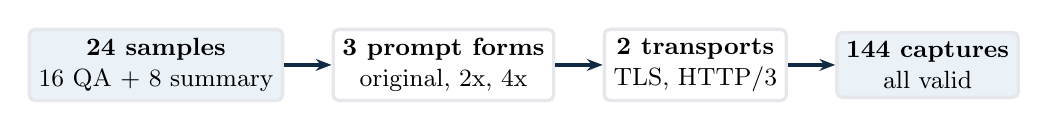
\begin{tikzpicture}[
  node distance=6mm,
  box/.style={rounded corners=2pt,draw=AIGrid,very thick,fill=white,
              minimum height=0.82cm,minimum width=2.2cm,align=center,font=\small},
  arrow/.style={-{Stealth[length=2mm]},very thick,color=ReportNavy}
]
  \node[box,fill=ReportLight] (data) {\bfseries 24 samples\\16 QA + 8 summary};
  \node[box,right=of data] (compress) {\bfseries 3 prompt forms\\original, 2x, 4x};
  \node[box,right=of compress] (protocol) {\bfseries 2 transports\\TLS, HTTP/3};
  \node[box,right=of protocol,fill=ReportLight] (capture) {\bfseries 144 captures\\all valid};
  \draw[arrow] (data) -- (compress);
  \draw[arrow] (compress) -- (protocol);
  \draw[arrow] (protocol) -- (capture);
\end{tikzpicture}
\end{center}

\begin{center}
\small
\renewcommand{\arraystretch}{1.22}
\begin{tabularx}{\linewidth}{@{}p{0.23\linewidth}Y@{}}
\toprule
\textbf{Setting} & \textbf{Value used in the baseline experiment} \\
\midrule
Target LLM & Qwen3.5-9B, served by vLLM \\
Hardware & Two GPU workers; each worker handled a disjoint sample shard \\
Decoding & Temperature 0, seed 42, thinking disabled \\
QA generation cap & 256 output tokens \\
Summary generation cap & 1,024 output tokens \\
Prompt conditions & No compression, LongLLMLingua 2x, LongLLMLingua 4x \\
TLS path & TLS 1.3 with HTTP/1.1 over TCP \\
QUIC path & HTTP/3 over QUIC \\
Capture unit & One request-response transaction per metric record \\
Network condition & Local loopback baseline with effectively zero added RTT \\
Repetitions & One completed repetition for each baseline cell \\
Primary metrics & Directional bytes, total bytes, packet count, elapsed time,
input/output tokens, and finish reason \\
\bottomrule
\end{tabularx}
\end{center}

\subsection{Run-count logic}

\[
  (16\ \mathrm{QA} + 8\ \mathrm{summary})
  \times 3\ \mathrm{prompt\ forms}
  \times 2\ \mathrm{transports}
  \times 1\ \mathrm{repeat}
  = \mathbf{144\ captures}
\]

The planned full controlled sweep expands to 52 workload items, two network
conditions, and three repetitions:
\[
  52 \times 3 \times 2 \times 2 \times 3 = \mathbf{1,872\ runs}.
\]

\subsection{How traffic is captured}

The local client sends the same OpenAI-compatible request payload through two
front-door listeners. Caddy terminates TLS 1.3 and forwards the unchanged
request to vLLM. TCP port 8443 carries HTTP/1.1; UDP port 8444 carries
HTTP/3-only QUIC traffic through an \texttt{aioquic} client. There is no TCP
fallback in the HTTP/3 condition.

\begin{center}
\small
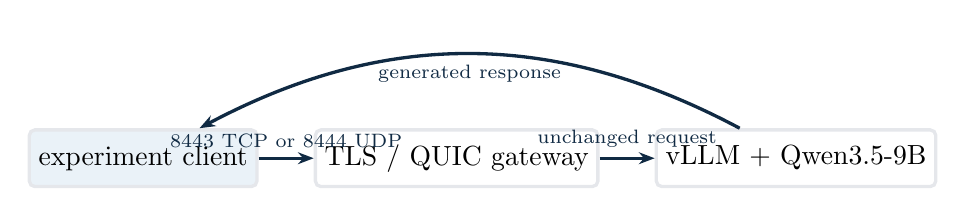
\begin{tikzpicture}[
  node distance=7mm,
  box/.style={rounded corners=2pt,draw=AIGrid,very thick,minimum height=0.72cm,
              minimum width=2.0cm,align=center},
  arrow/.style={-{Stealth[length=2mm]},very thick,color=ReportNavy}
]
  \node[box,fill=ReportLight] (client) {experiment client};
  \node[box,right=of client] (caddy) {TLS / QUIC gateway};
  \node[box,right=of caddy] (vllm) {vLLM + Qwen3.5-9B};
  \draw[arrow] (client) -- node[above,font=\scriptsize]{8443 TCP or 8444 UDP} (caddy);
  \draw[arrow] (caddy) -- node[above,font=\scriptsize]{unchanged request} (vllm);
  \draw[arrow,bend right=28] (vllm) to node[below,font=\scriptsize]{generated response} (client);
\end{tikzpicture}
\end{center}

\texttt{dumpcap} performs lightweight acquisition and writes one
\texttt{pcapng} file per request. \texttt{tshark} then calculates directional
bytes, total frame bytes, packet counts, and protocol evidence offline. This
separates acquisition from analysis and permits metrics to be regenerated
without repeating GPU inference.

\subsection{How model randomness and multi-turn dependence are controlled}

\begin{itemize}
  \item Temperature 0 and seed 42 reduce decoding variability.
  \item Every condition receives the same frozen conversation and task
        instruction; only the prompt representation changes.
  \item QA tasks do not create a new branching conversation. Each question is
        evaluated independently against the original recorded LoCoMo history.
  \item Event summarization similarly requests a fixed speaker-level artifact
        from the recorded history. It does not feed a generated answer into the
        next sample.
  \item The measured response is retained with its token count and finish
        reason, so unexpectedly short or truncated outputs can be identified.
\end{itemize}

\resultpage{Compression reaches distinct token budgets}{
LongLLMLingua produced clearly separated prompt sizes for both tasks. This
confirms that the requested conditions are operationally distinct before any
traffic comparison is made.
}{0.78}{\PlotTokenMedians}

\begin{center}
\small
\begin{tabular}{@{}lrrr@{}}
\toprule
\textbf{Workload} & \textbf{Original} & \textbf{2x} & \textbf{4x} \\
\midrule
QA median input tokens & 45,752 & 18,568 & 9,650 \\
Event-summary median input tokens & 35,326 & 14,204 & 7,950 \\
\bottomrule
\end{tabular}
\end{center}
\tablesource{Table 1. Median input-token counts. Transport is omitted because
the same prompt is used for both transport paths.}

\resultpage{Upload traffic falls after prompt compression}{
Client-to-server traffic follows the reduced prompt size closely. The result
is consistent across TLS 1.3 and HTTP/3.
}{0.88}{\PlotUploadReduction}

\begin{center}
\small
\begin{tabular}{@{}llrr@{}}
\toprule
\textbf{Workload} & \textbf{Transport} & \textbf{2x reduction} & \textbf{4x reduction} \\
\midrule
QA & TLS 1.3 & 53.6\% & 75.6\% \\
QA & HTTP/3 & 54.2\% & 76.1\% \\
Event summary & TLS 1.3 & 38.0\% & 55.2\% \\
Event summary & HTTP/3 & 37.8\% & 54.8\% \\
\bottomrule
\end{tabular}
\end{center}
\tablesource{Table 2. Paired median reduction in client-to-server bytes versus
the original prompt. Whiskers in the figure are bootstrap 95\% confidence intervals.}

\resultpage{Total traffic reduction depends on workload direction}{
For QA, upload dominates and the traffic benefit survives end-to-end. For
event summarization, long generated responses dilute the benefit of reducing
the prompt.
}{0.88}{\PlotTotalReduction}

\begin{center}
\small
\begin{tabular}{@{}llrr@{}}
\toprule
\textbf{Workload} & \textbf{Transport} & \textbf{2x reduction} & \textbf{4x reduction} \\
\midrule
QA & TLS 1.3 & 51.5\% & 71.2\% \\
QA & HTTP/3 & 52.7\% & 72.9\% \\
Event summary & TLS 1.3 & 6.2\% & 19.7\% \\
Event summary & HTTP/3 & 6.9\% & 22.0\% \\
\bottomrule
\end{tabular}
\end{center}
\tablesource{Table 3. Paired median reduction in bidirectional frame bytes.}

\resultpage{QA is an input-dominated exchange}{
The uploaded conversation is the largest component of QA traffic. Output
answers are short, so prompt compression removes most of the transmitted
payload.
}{0.82}{\PlotDirectionQA}

\begin{center}
\scriptsize
\begin{tabular}{@{}llrrr@{}}
\toprule
\textbf{Transport} & \textbf{Prompt} & \textbf{Upload (KiB)} &
\textbf{Download (KiB)} & \textbf{Total (KiB)} \\
\midrule
TLS 1.3 & Original & 142.8 & 6.9 & 147.9 \\
TLS 1.3 & 2x & 52.7 & 7.0 & 62.2 \\
TLS 1.3 & 4x & 32.4 & 7.2 & 41.1 \\
HTTP/3 & Original & 150.0 & 5.2 & 154.2 \\
HTTP/3 & 2x & 54.6 & 4.9 & 62.3 \\
HTTP/3 & 4x & 33.2 & 5.7 & 39.8 \\
\bottomrule
\end{tabular}
\end{center}
\tablesource{Table 4. Median directional and total captured bytes for QA.}

\resultpage{Event summaries are output-dominated exchanges}{
Compression still reduces upload traffic, but the generated summary remains
roughly 220--255 KiB. Slightly longer compressed-prompt outputs further limit
total-byte savings.
}{0.82}{\PlotDirectionSummary}

\begin{center}
\scriptsize
\begin{tabular}{@{}llrrr@{}}
\toprule
\textbf{Transport} & \textbf{Prompt} & \textbf{Upload (KiB)} &
\textbf{Download (KiB)} & \textbf{Total (KiB)} \\
\midrule
TLS 1.3 & Original & 155.6 & 221.8 & 378.2 \\
TLS 1.3 & 2x & 97.7 & 246.1 & 342.6 \\
TLS 1.3 & 4x & 79.3 & 248.6 & 330.5 \\
HTTP/3 & Original & 165.4 & 215.2 & 381.7 \\
HTTP/3 & 2x & 104.8 & 237.7 & 342.5 \\
HTTP/3 & 4x & 85.6 & 238.0 & 326.1 \\
\bottomrule
\end{tabular}
\end{center}
\tablesource{Table 5. Median directional and total captured bytes for event summaries.}

\resultpage{TLS and HTTP/3 transfer similar total bytes}{
On the zero-RTT loopback baseline, all median HTTP/3-to-TLS total-byte ratios
remain within four percent of parity.
}{0.78}{\PlotProtocolBytes}

\begin{center}
\small
\begin{tabular}{@{}lrrr@{}}
\toprule
\textbf{Workload} & \textbf{Original} & \textbf{2x} & \textbf{4x} \\
\midrule
QA: HTTP/3 / TLS total bytes & 1.04 & 1.00 & 0.97 \\
Summary: HTTP/3 / TLS total bytes & 1.01 & 0.99 & 0.99 \\
\bottomrule
\end{tabular}
\end{center}
\tablesource{Table 6. Paired median protocol ratios. A ratio of 1.00 indicates parity.}

\resultpage{HTTP/3 packetization is visible for short QA}{
HTTP/3 sends more captured packets for the short QA exchange, especially for
the original long prompt. This difference narrows as compression reduces the
payload. Summary packet counts are close between transports.
}{0.78}{\PlotProtocolPackets}

\begin{center}
\small
\begin{tabular}{@{}lrrr@{}}
\toprule
\textbf{Workload} & \textbf{Original} & \textbf{2x} & \textbf{4x} \\
\midrule
QA: HTTP/3 / TLS packets & 2.92 & 1.57 & 1.17 \\
Summary: HTTP/3 / TLS packets & 1.07 & 1.02 & 1.01 \\
\bottomrule
\end{tabular}
\end{center}
\tablesource{Table 7. Paired median packet-count ratios.}

\resultpage{Latency follows the amount of input processed}{
QA latency falls strongly because the target model processes far fewer input
tokens. Summary latency falls less because response generation remains the
dominant computation.
}{0.88}{\PlotLatencyMedians}

\begin{center}
\small
\begin{tabular}{@{}llrrr@{}}
\toprule
\textbf{Workload} & \textbf{Transport} & \textbf{Original} & \textbf{2x} & \textbf{4x} \\
\midrule
QA & TLS 1.3 & 8.64 s & 3.43 s & 1.95 s \\
QA & HTTP/3 & 8.64 s & 3.42 s & 1.95 s \\
Event summary & TLS 1.3 & 24.04 s & 21.23 s & 20.75 s \\
Event summary & HTTP/3 & 24.05 s & 21.24 s & 20.77 s \\
\bottomrule
\end{tabular}
\end{center}
\tablesource{Table 8. Median end-to-end generation latency.}

\clearpage
\section{Interpretation, research standard, and next actions}

\subsection{What the pilot establishes}

\begin{enumerate}
  \item \textbf{The measurement chain works end-to-end.} Compression, local
        inference, encrypted transmission, packet capture, metric extraction,
        retry, and resume all produced a complete baseline matrix.
  \item \textbf{Network savings are workload-dependent.} A compression ratio
        alone does not determine total savings; the relative size of request
        and response traffic matters.
  \item \textbf{The transport baseline is controlled.} TLS and HTTP/3 receive
        the same semantic input and model configuration, enabling paired
        comparison.
  \item \textbf{The current results are preliminary, not a final
        network-condition claim.} They represent one loopback repetition and
        should be treated as an effect-discovery and pipeline-validation study.
\end{enumerate}

\subsection{Recommended full experiment}

\begin{center}
\renewcommand{\arraystretch}{1.25}
\begin{tabularx}{\linewidth}{@{}p{0.25\linewidth}Y@{}}
\toprule
\textbf{Factor} & \textbf{Recommended setting} \\
\midrule
Workloads & 52 total workload items, retaining both QA and event summarization \\
Compression & Original, LongLLMLingua 2x, LongLLMLingua 4x \\
Transports & TLS 1.3 / HTTP/1.1 and HTTP/3 / QUIC \\
Network conditions & Controlled loopback plus one realistic RTT condition \\
RTT treatment & Fixed delay applied symmetrically and reported explicitly \\
MTU & Fixed value matched across transports and documented with the result \\
Offloads & Disable segmentation and aggregation offloads during capture \\
Connection state & Report whether measurements use warm persistent connections
or cold per-request connections; do not mix them in one estimate \\
Repetitions & Three independent repetitions per experiment cell \\
Primary analysis & Paired medians, dispersion or confidence intervals, and
per-sample ratios \\
\bottomrule
\end{tabularx}
\end{center}

\subsection{Why three repetitions are defensible}

Three repetitions are a practical minimum for a costly GPU and packet-capture
experiment. They permit variability checks and paired aggregation without the
cost of ten repetitions. For a top-tier submission, the report should show
confidence intervals, disclose that repetitions are limited, and emphasize
effect sizes rather than relying only on significance tests. Sample diversity
across 52 workload items contributes more evidence than repeatedly measuring a
small number of prompts ten times.

\subsection{Resume and partial-result strategy}

The runner should treat each combination of sample, compression condition,
transport, network condition, and repetition as a unique job key. A completed
job is appended atomically to the result artifact. On restart, existing valid
keys are skipped, failed keys are re-queued, and new results are merged without
overwriting the 144 baseline records. This permits a two-hour partial run for a
presentation while preserving all work for later continuation.

\clearpage
\section{Figure-selection guide}

The separate figure catalog contains thirteen candidate views. The following
subset is recommended for the main paper or presentation.

\begin{center}
\small
\renewcommand{\arraystretch}{1.25}
\begin{tabularx}{\linewidth}{@{}p{0.10\linewidth}p{0.29\linewidth}Y@{}}
\toprule
\textbf{Figure} & \textbf{Purpose} & \textbf{Recommendation} \\
\midrule
F1 & Input-token medians & Keep as a setup validation figure or appendix item. \\
F2 & Upload-byte reduction & Keep; this directly answers the traffic question. \\
F3 & Total-byte reduction & Keep; this is the clearest primary result. \\
F4--F5 & Directional stacked bytes & Keep both or combine as a two-panel figure;
they explain the workload-dependent effect. \\
F6 & HTTP/3-to-TLS byte ratio & Keep for the protocol comparison. \\
F7 & HTTP/3-to-TLS packet ratio & Keep if packetization is a research question;
otherwise move to the appendix. \\
F8 & Absolute latency & Keep if system performance is discussed. \\
F9 & Token/upload scatter & Strong appendix evidence for the $r=0.88$ relation. \\
F10 & Paired ECDF & Best paper-style distribution figure; keep in the paper. \\
F11--F13 & Output share, absolute traffic, latency reduction & Useful alternate
views; choose only one to avoid repeating the same conclusion. \\
\bottomrule
\end{tabularx}
\end{center}

\section{References and reproducibility}

\begin{itemize}
  \item Pan et al. ``LLMLingua-2: Data Distillation for Efficient and Faithful
        Task-Agnostic Prompt Compression.'' arXiv:2403.12968, 2024.
  \item Maharana et al. ``Evaluating Very Long-Term Conversational Memory of
        LLM Agents.'' Proceedings of ACL 2024.
  \item Metric artifact:
        \texttt{artifacts/preliminary\_metrics\_baseline.csv}.
  \item Analysis:
        \texttt{analysis/prepare\_figure\_data.py}.
  \item Figure definitions:
        \texttt{figures/conference\_plots.tex}.
\end{itemize}

All numerical claims in this report are computed from the 144 valid baseline
captures. Tables use medians unless explicitly described as paired median
ratios. Bootstrap confidence intervals use a fixed random seed for
reproducibility.

\end{document}
